% Chapter 2

\chapter{Diseño del experimento}
\label{Chap:DisExp} % For referencing the chapter elsewhere, use \ref{Chapter2} 

%----------------------------------------------------------------------------------------

\section{Introducción}

En este capítulo, se muestra a detalle la prueba a la que será sometido el equipo de posicionamiento RTK implementado en la BeagleBone, así como la justificación de dicho experimento y se plantean las medidas que se tomarán para conocer la precisión que el sistema tiene.

\section{Bosquejo del experimento}

El sistema Real-Time Kinematics ofrece una precisión medible en distancia. Por lo tanto, se pretende dibujar una figura geométrica (cuadrado) de medidas conocidas en una determinada área donde las antenas de GPS estén de la forma menos afectada posible por interferencias como las planteadas en el marco teórico en la sección~\ref{subsec:CauErr} en la página~\pageref{subsec:CauErr}. Por tanto, se utiliza la siguiente técnica para el trazado de la figura:

\subsection{Bosquejo de la figura}

\begin{figure}[H]
\centering
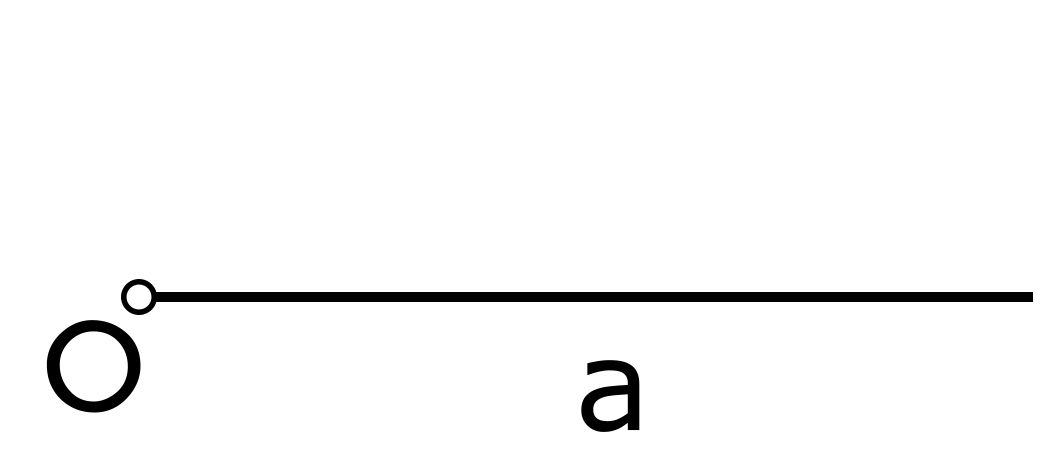
\includegraphics[width=0.95\textwidth]{Figures/Cuad1}
\caption[Primer paso del trazado de la figura.]{Primer paso del trazado de la figura.}
\label{fig:TrazFig1}
\end{figure}

Se traza una línea recta de medida $a$. En la figura~\ref{fig:TrazFig1}, la \textbf{O} indica el punto de origen del recorrido a seguir.\\

\begin{figure}[H]
\centering
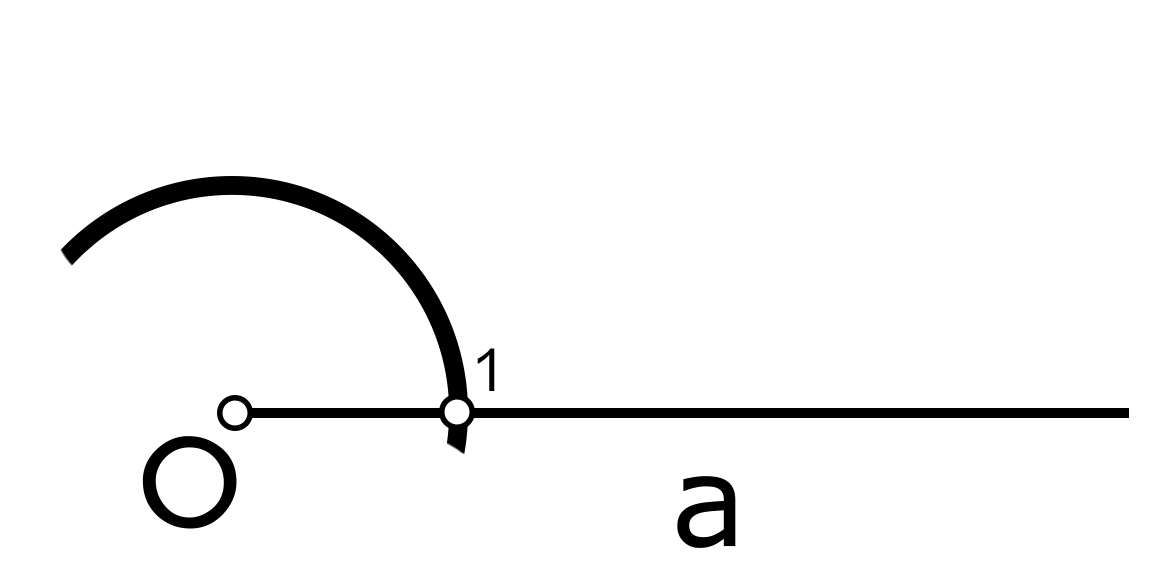
\includegraphics[width=0.95\textwidth]{Figures/Cuad2}
\caption[Primer arco de circunferencia.]{Primer arco de circunferencia.}
\label{fig:TrazFig2}
\end{figure}

Utilizando una cuerda tensa, ahora se dibuja un segmento de circunferencia o arco teniendo como centro al origen \textbf{O} y un radio arbitrario $r$ que debe de mantenerse constante, tal y como muestra la figura~\ref{fig:TrazFig2}. El punto donde el arco interseca a la primera línea será llamado punto 1. 

\begin{figure}[H]
\centering
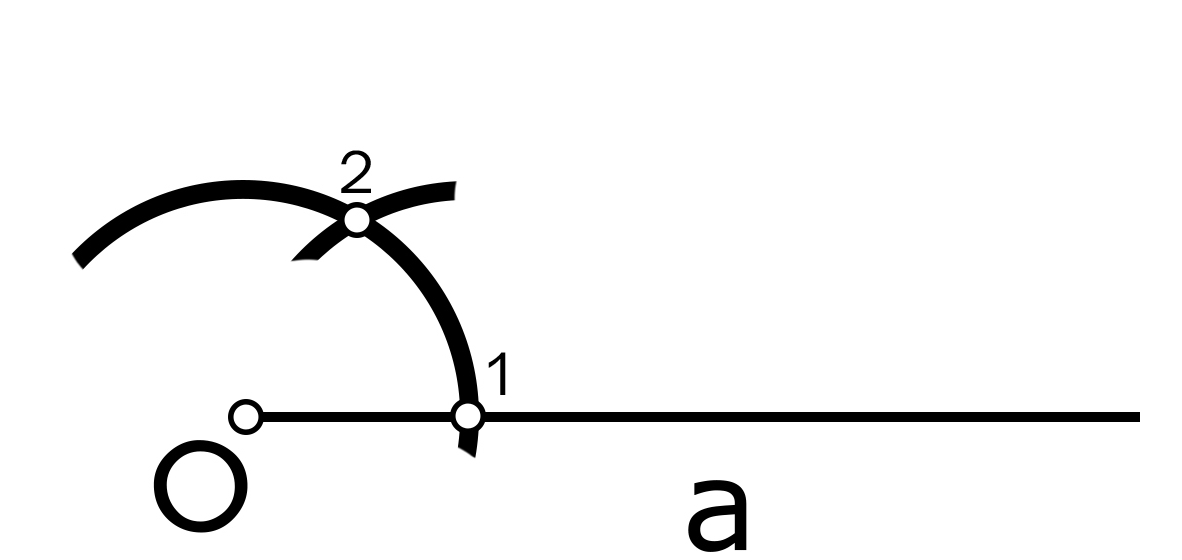
\includegraphics[width=0.95\textwidth]{Figures/Cuad3}
\caption[Segundo arco de circunferencia.]{Segundo arco de circunferencia.}
\label{fig:TrazFig3}
\end{figure}

Se trazará otro arco, manteniendo el mismo radio $r$, pero ahora teniendo como origen de la circunferencia al punto que se denotó como 1, como sugiere la figura~\ref{fig:TrazFig3}. Al punto de la intersección de los dos arcos dibujados anteriormente se le llamará punto 2.

\begin{figure}[H]
\centering
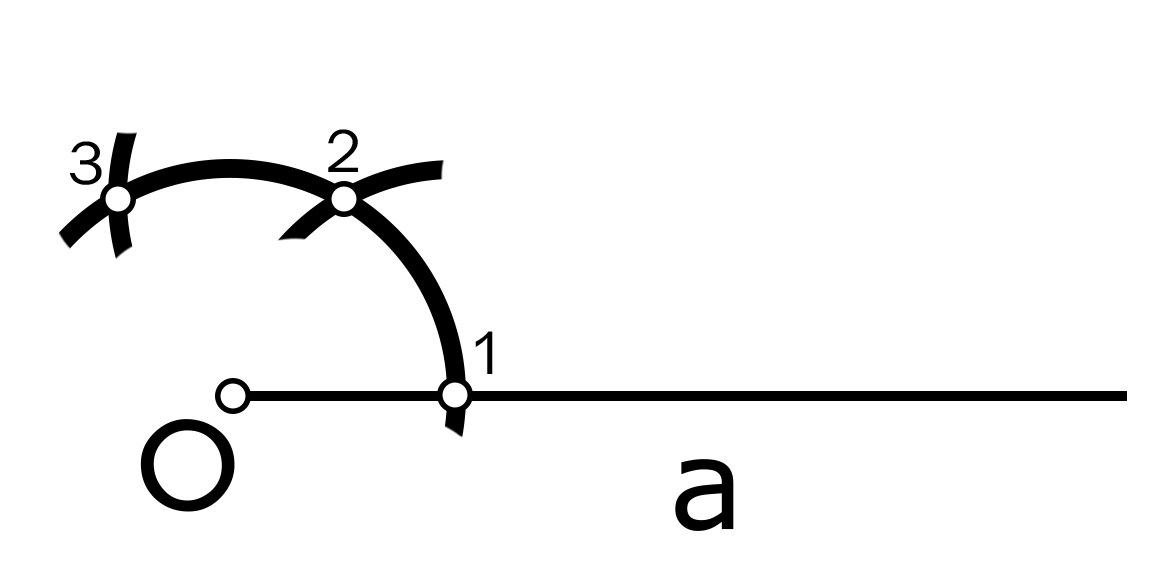
\includegraphics[width=0.95\textwidth]{Figures/Cuad4}
\caption[Tercer arco de circunferencia.]{Tercer arco de circunferencia.}
\label{fig:TrazFig4}
\end{figure}

Se repite el paso anterior con el arco de radio $r$, tomando como origen al punto 2, y buscando intersecarse con el primer arco de circunferencia trazado, como muestra la figura~\ref{fig:TrazFig4}. Al punto de intersección se le llamará punto 3.

\begin{figure}[H]
\centering
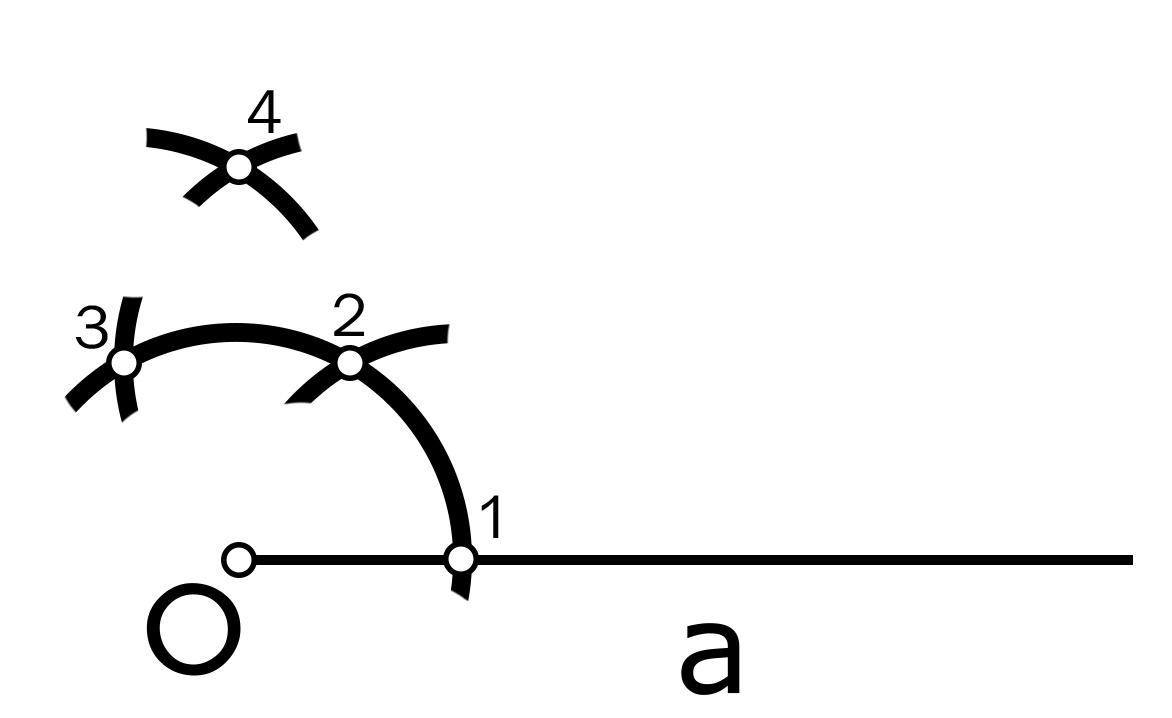
\includegraphics[width=0.95\textwidth]{Figures/Cuad5}
\caption[Cuarto y quinto arco de circunferencia.]{Cuarto y quinto arco de circunferencia.}
\label{fig:TrazFig5}
\end{figure}

Ahora, con dos arcos de circunferencia de radio $r$, pero con orígenes en los puntos 2 y 3, se trata de localizar un cuarto punto tal que, trazando una recta entre el punto de origen y esta cuarta marca, el segmento dibujado sea perpendicular a la recta original de tamaño $a$ dibujada al principio. Lo anterior se logra trazando los arcos que marca el punto número 4 en la figura~\ref{fig:TrazFig5}.

\begin{figure}[H]
\centering
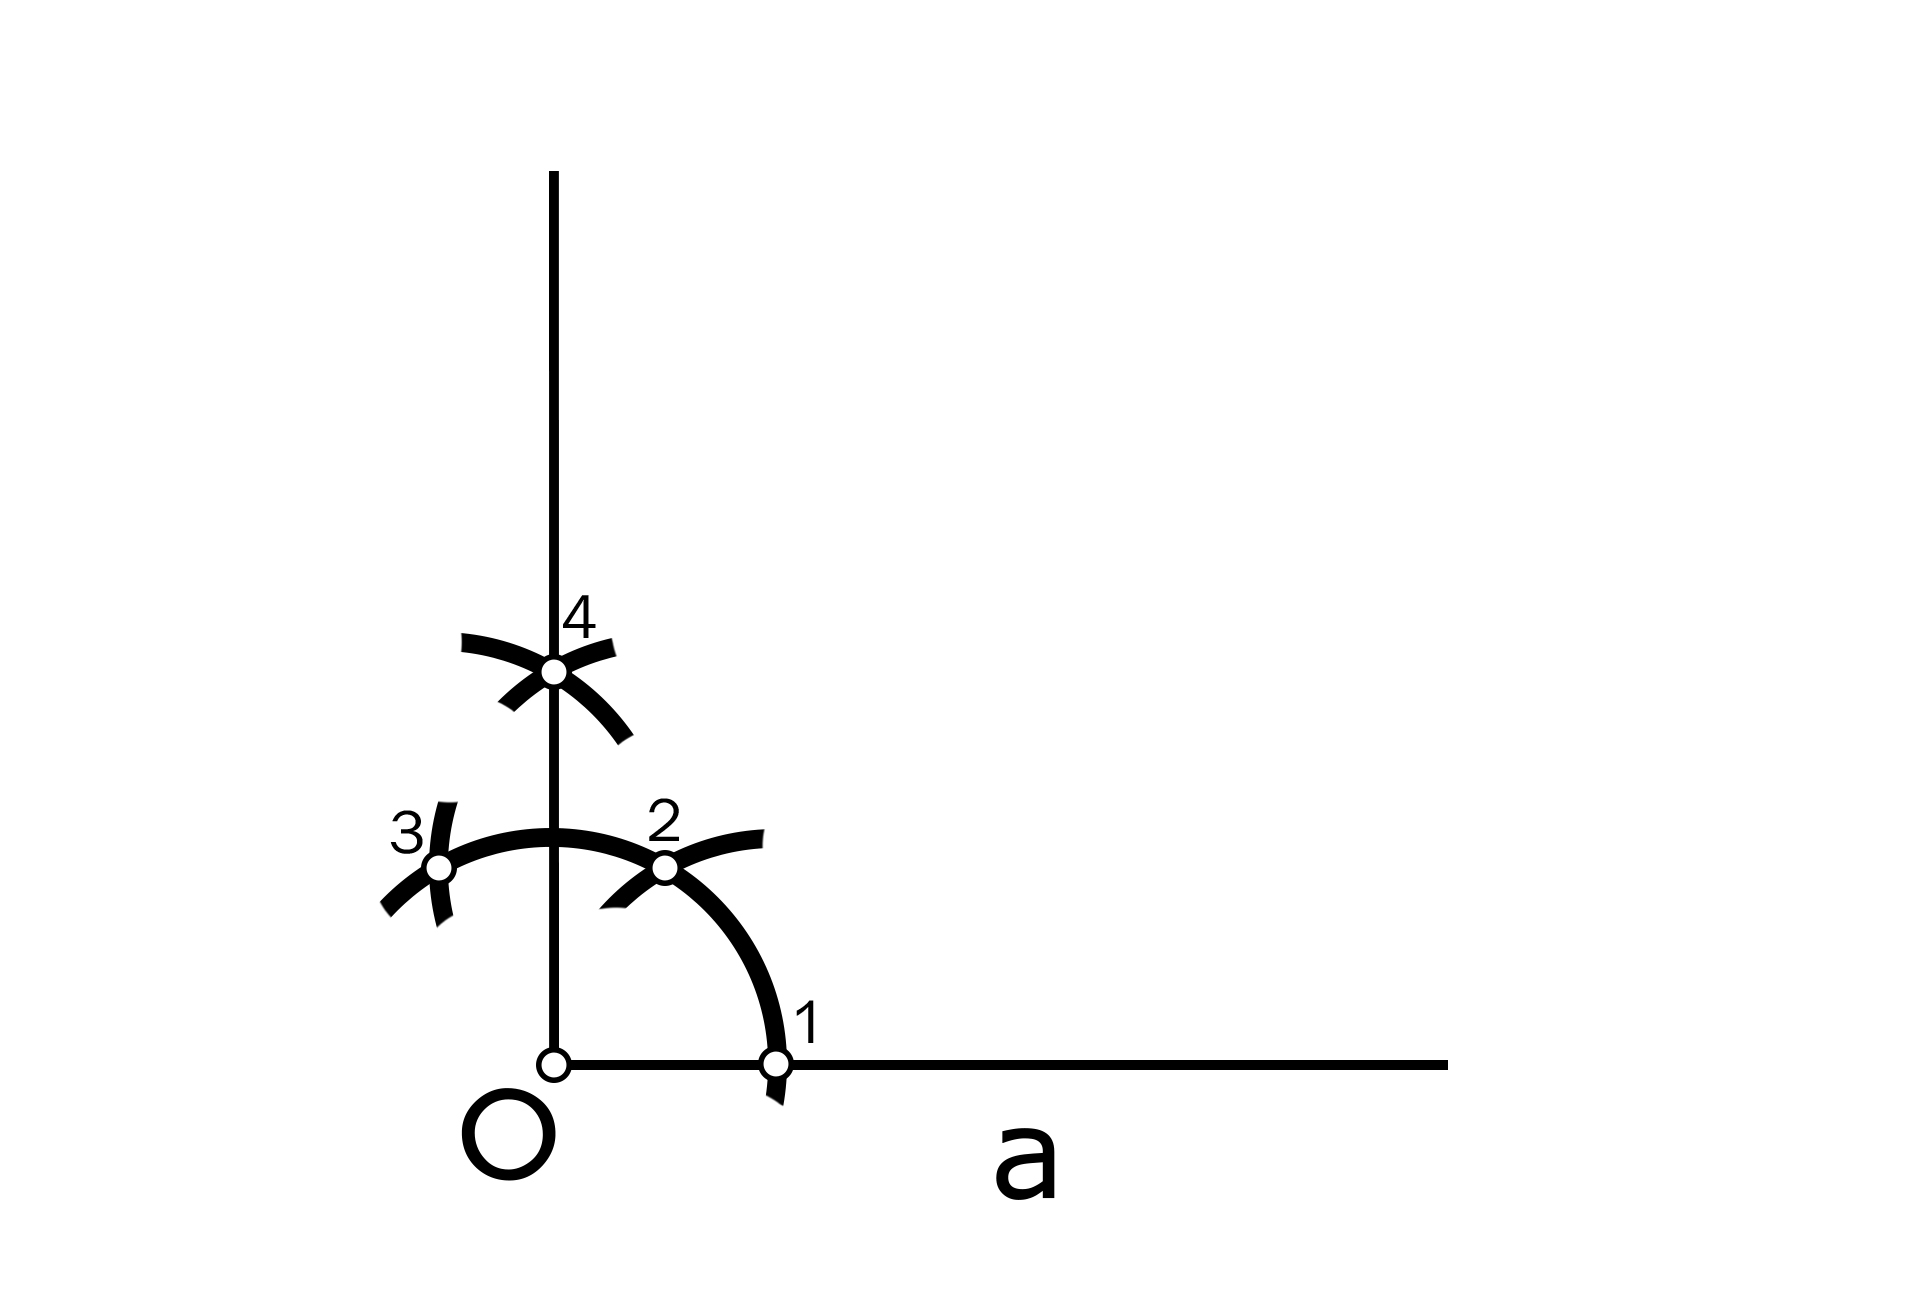
\includegraphics[width=0.95\textwidth]{Figures/Cuad6}
\caption[Segundo lado del cuerpo geométrico.]{Segundo lado del cuerpo geométrico.}
\label{fig:TrazFig6}
\end{figure}

Así, se traza una recta entre el punto 4 y el origen \textbf{O} para obtener el segundo lado de la figura geométrica a utilizar, como indica la figura~\ref{fig:TrazFig6}. Los anteriores pasos se repiten simétricamente en el otro extremo de la recta inicial de tamaño $a$ para obtener el tercer lado del cuerpo geométrico, como muestra la figura~\ref{fig:TrazFig7}.

\begin{figure}[H]
\centering
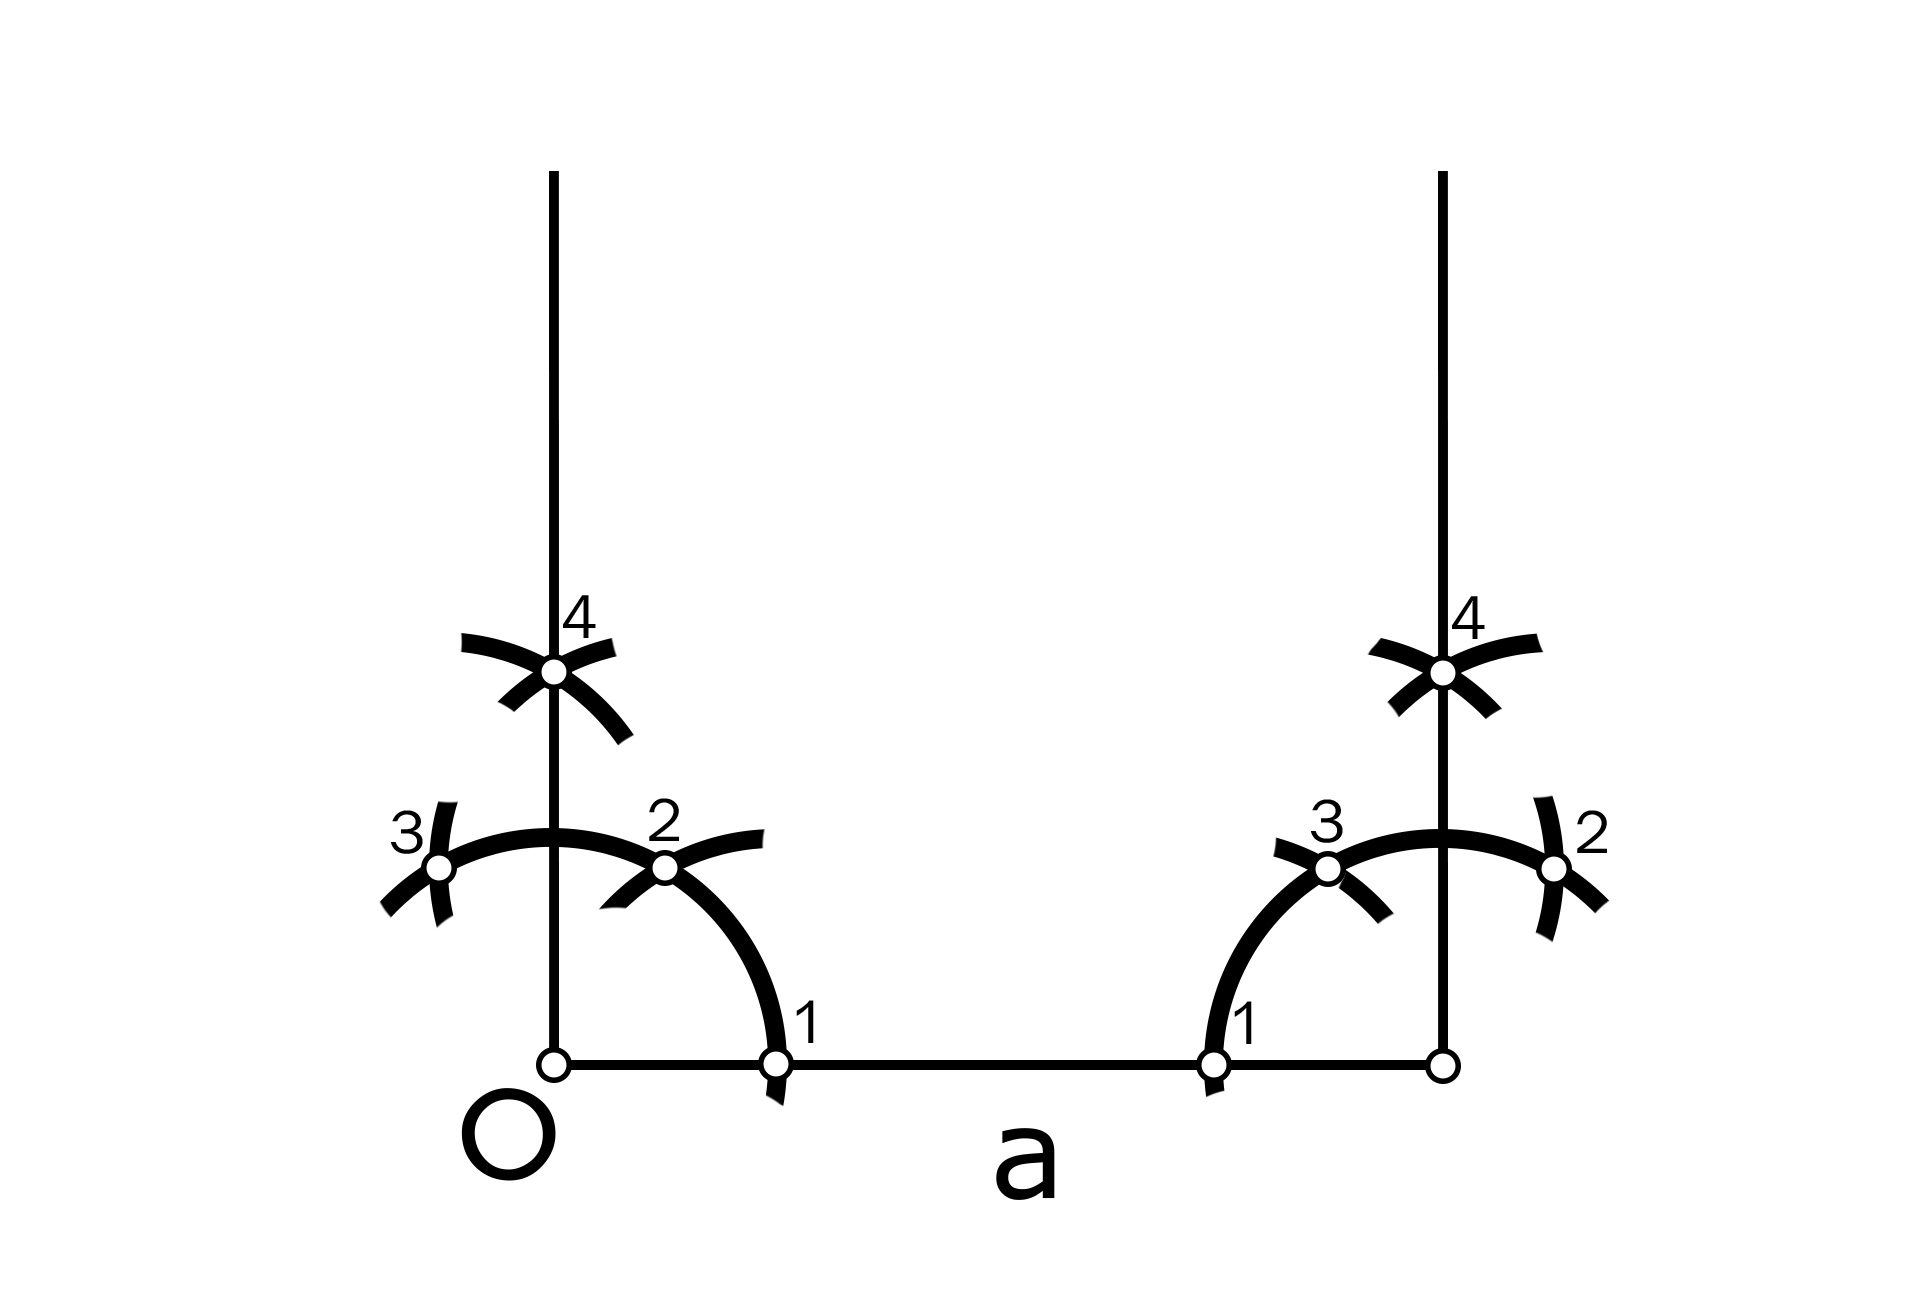
\includegraphics[width=0.95\textwidth]{Figures/Cuad7}
\caption[Tercer lado del cuerpo geométrico.]{Tercer lado del cuerpo geométrico.}
\label{fig:TrazFig7}
\end{figure}

Para garantizar que las medidas de los segmentos obtenidos en estos últimos pasos correspondan con el primer segmento $a$, se trazará nuevamente otro arco, pero ahora de radio $a$ y centrado en el punto de origen \textbf{O}, de forma que el arco a trazar se interseque con el lado perpendicular a la recta y que está sobre el origen, tal y como sugiere la figura~\ref{fig:TrazFig8}. El segmento acotado tendrá $a$ como medida. 

\begin{figure}[H]
\centering
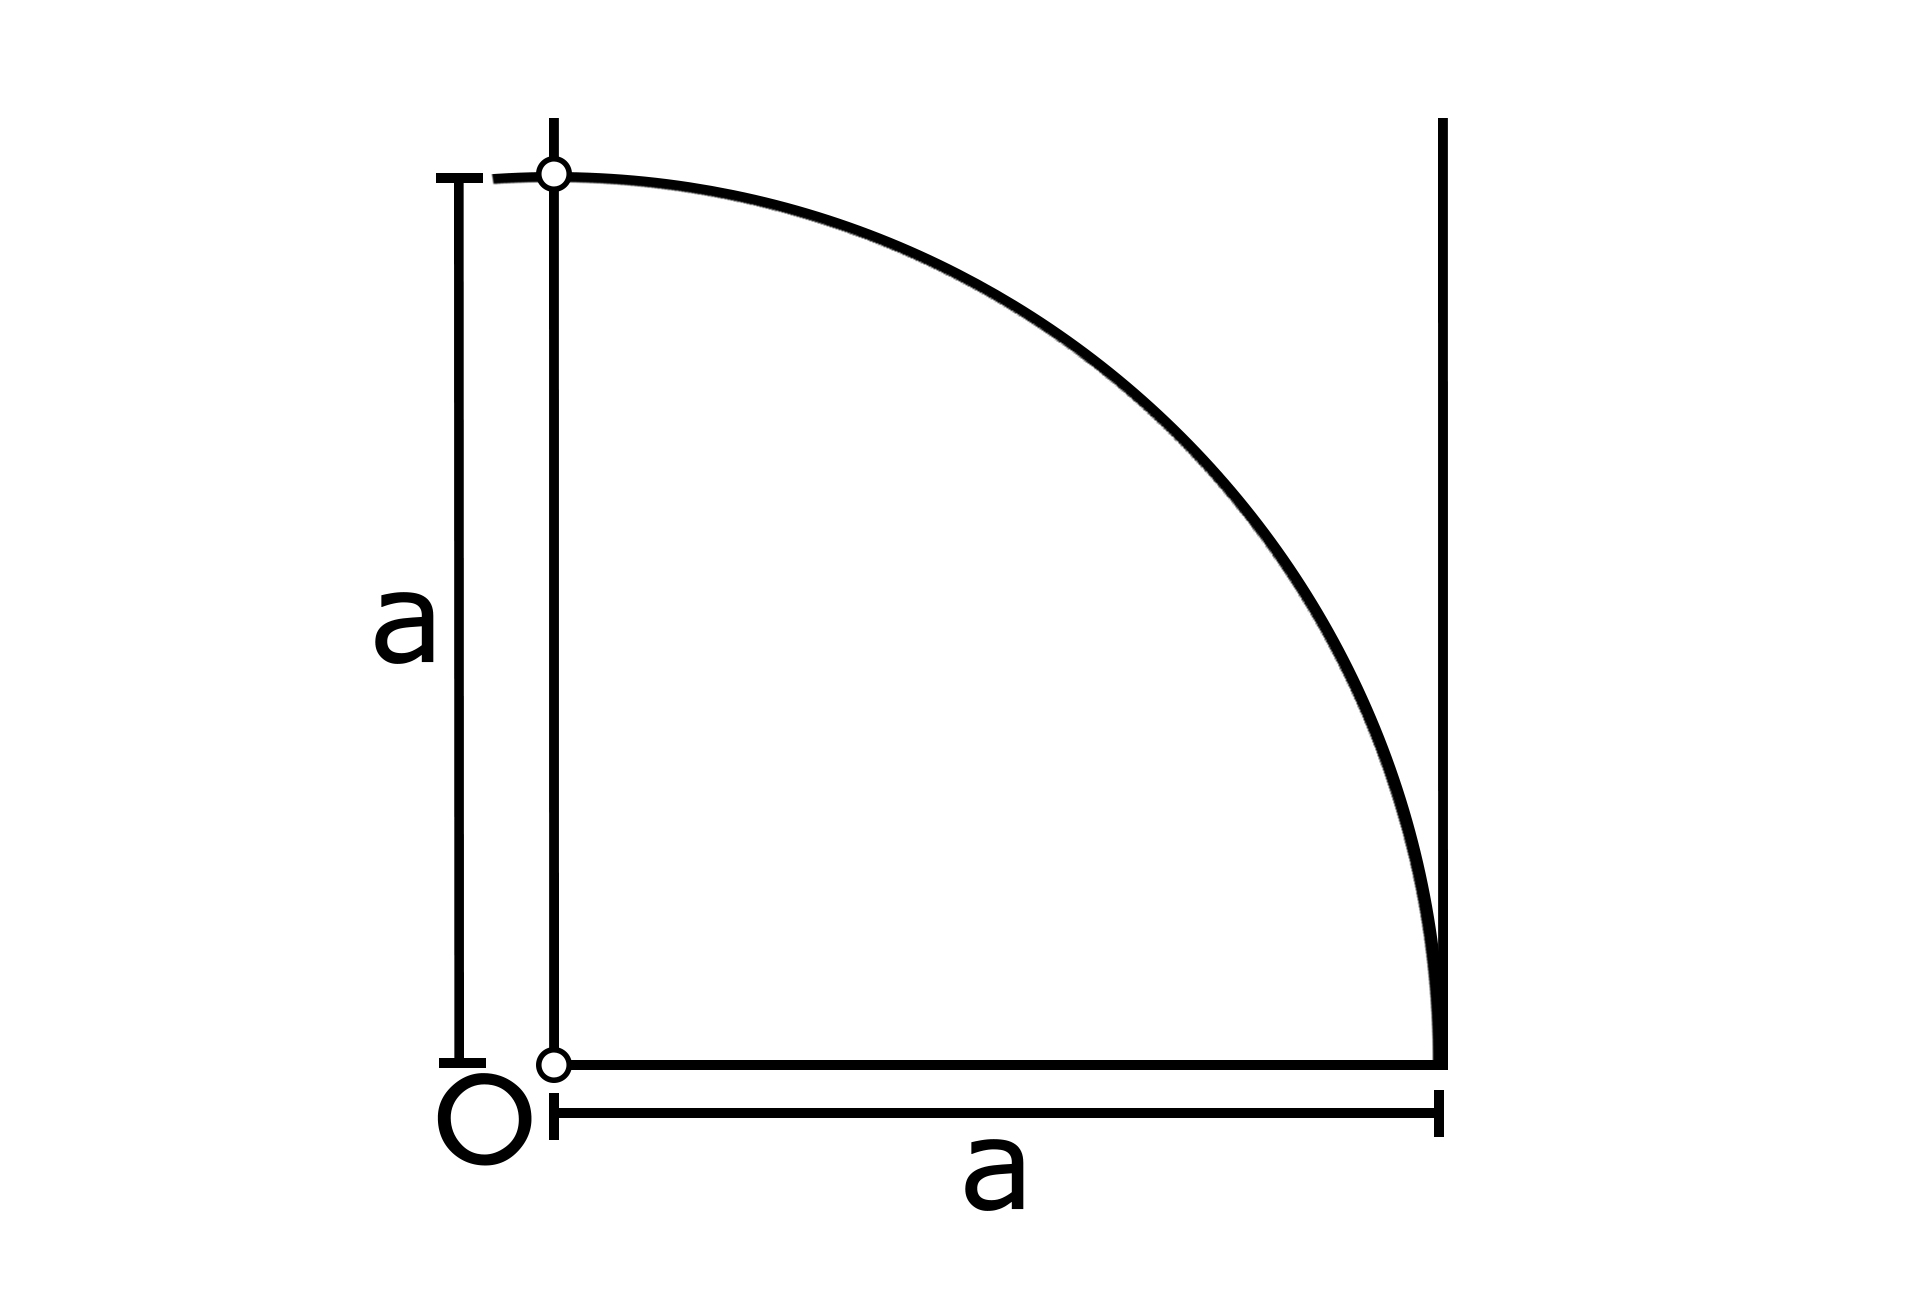
\includegraphics[width=0.95\textwidth]{Figures/Cuad8}
\caption[Acotamiento del segundo lado de la figura.]{Acotamiento del segundo lado de la figura.}
\label{fig:TrazFig8}
\end{figure}

El paso anterior se repite de forma simétrica en el otro extremo del primer segmento dibujado, como indica la figura~\ref{fig:TrazFig9}.

\begin{figure}[H]
\centering
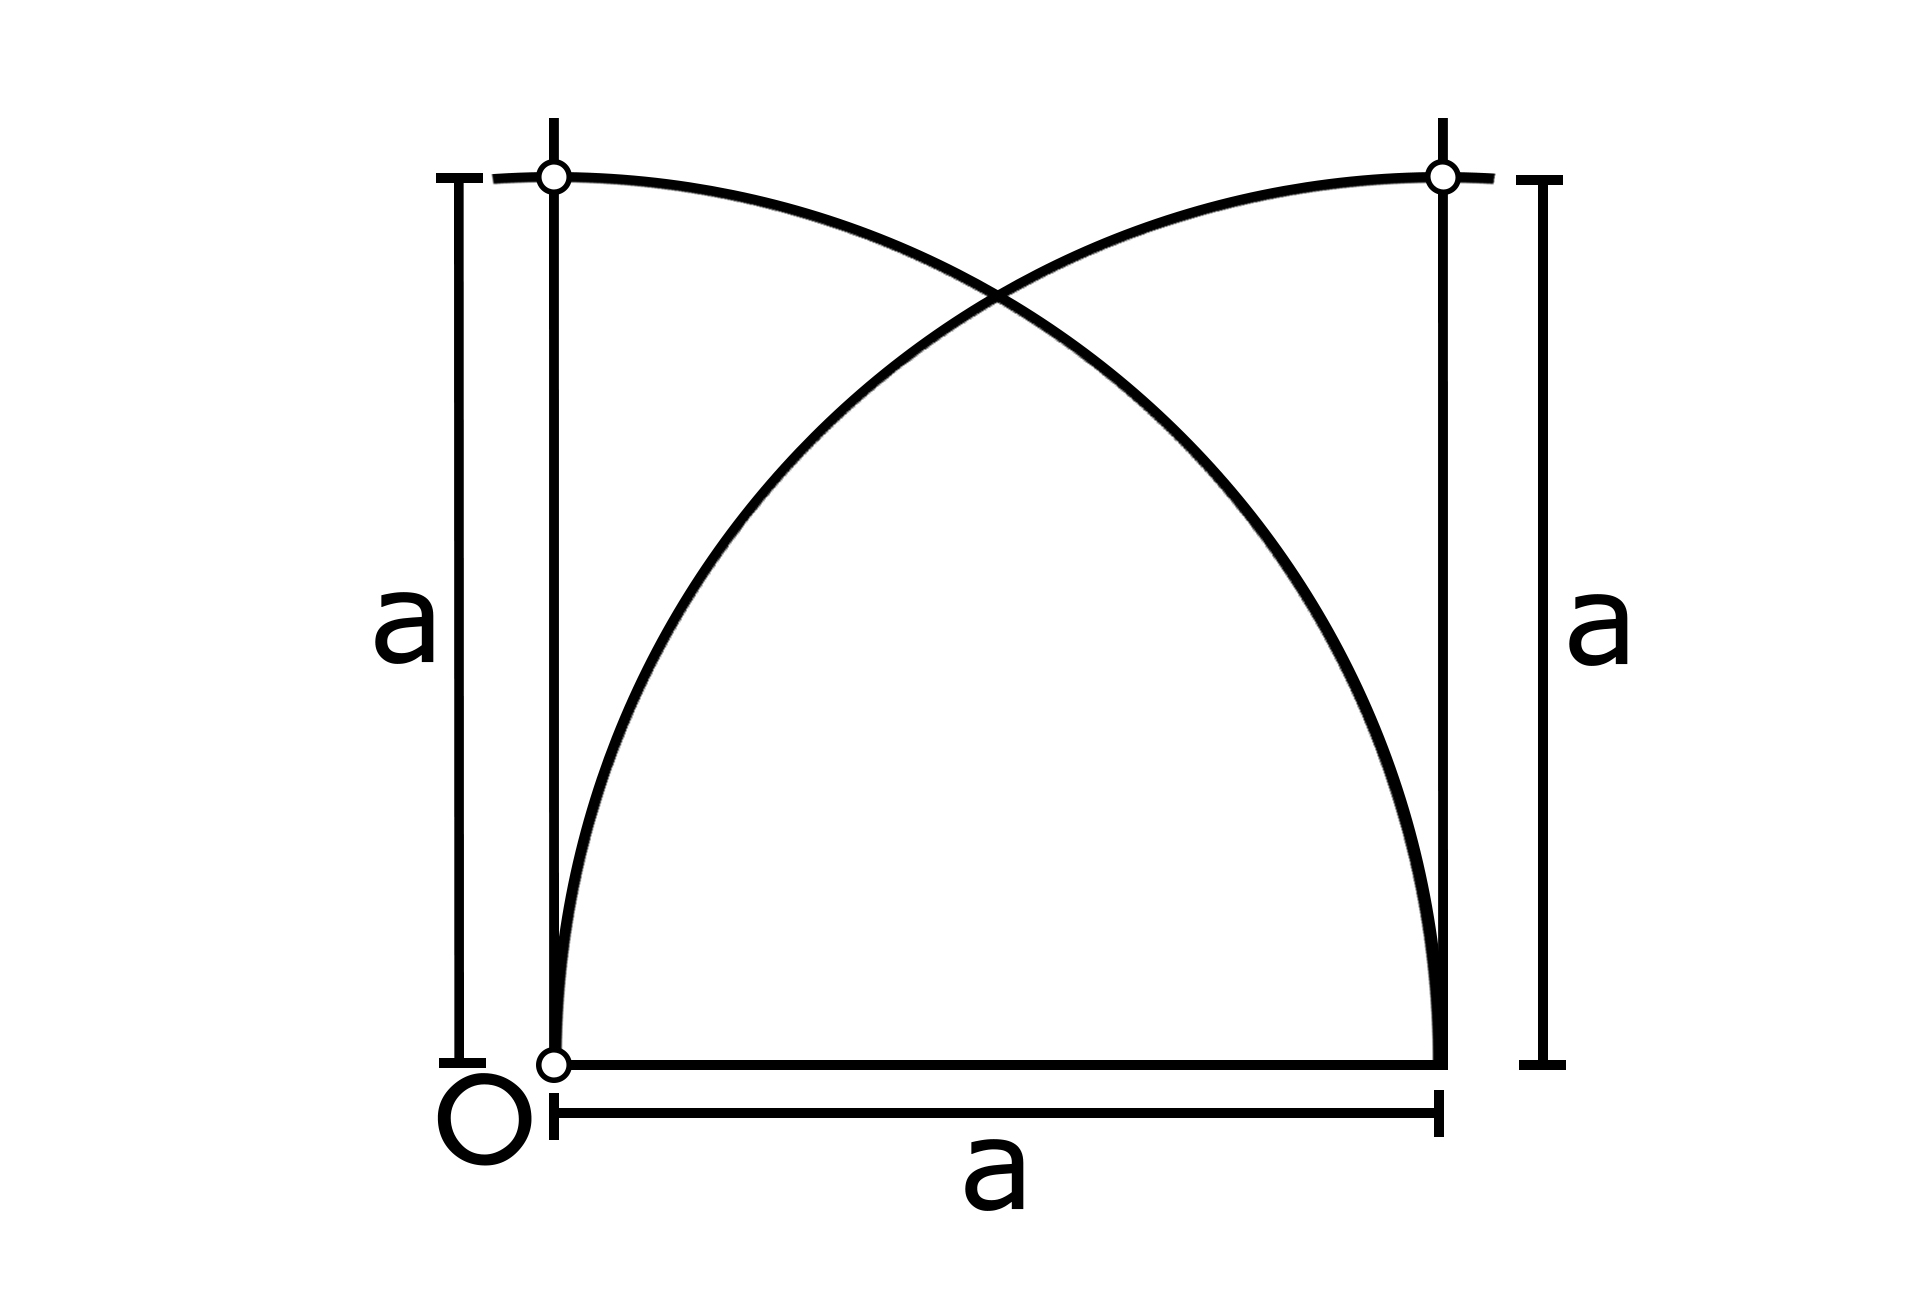
\includegraphics[width=0.95\textwidth]{Figures/Cuad9}
\caption[Acotamiento del tercer lado de la figura.]{Acotamiento del tercer lado de la figura.}
\label{fig:TrazFig9}
\end{figure}

Para obtener el último lado de la figura geométrica, basta con trazar un segmento de recta entre los puntos que acotaron las dos rectas anteriores, como indica la figura~\ref{fig:TrazFig10}. Ese segmento tendrá $a$ como medida.

\begin{figure}[H]
\centering
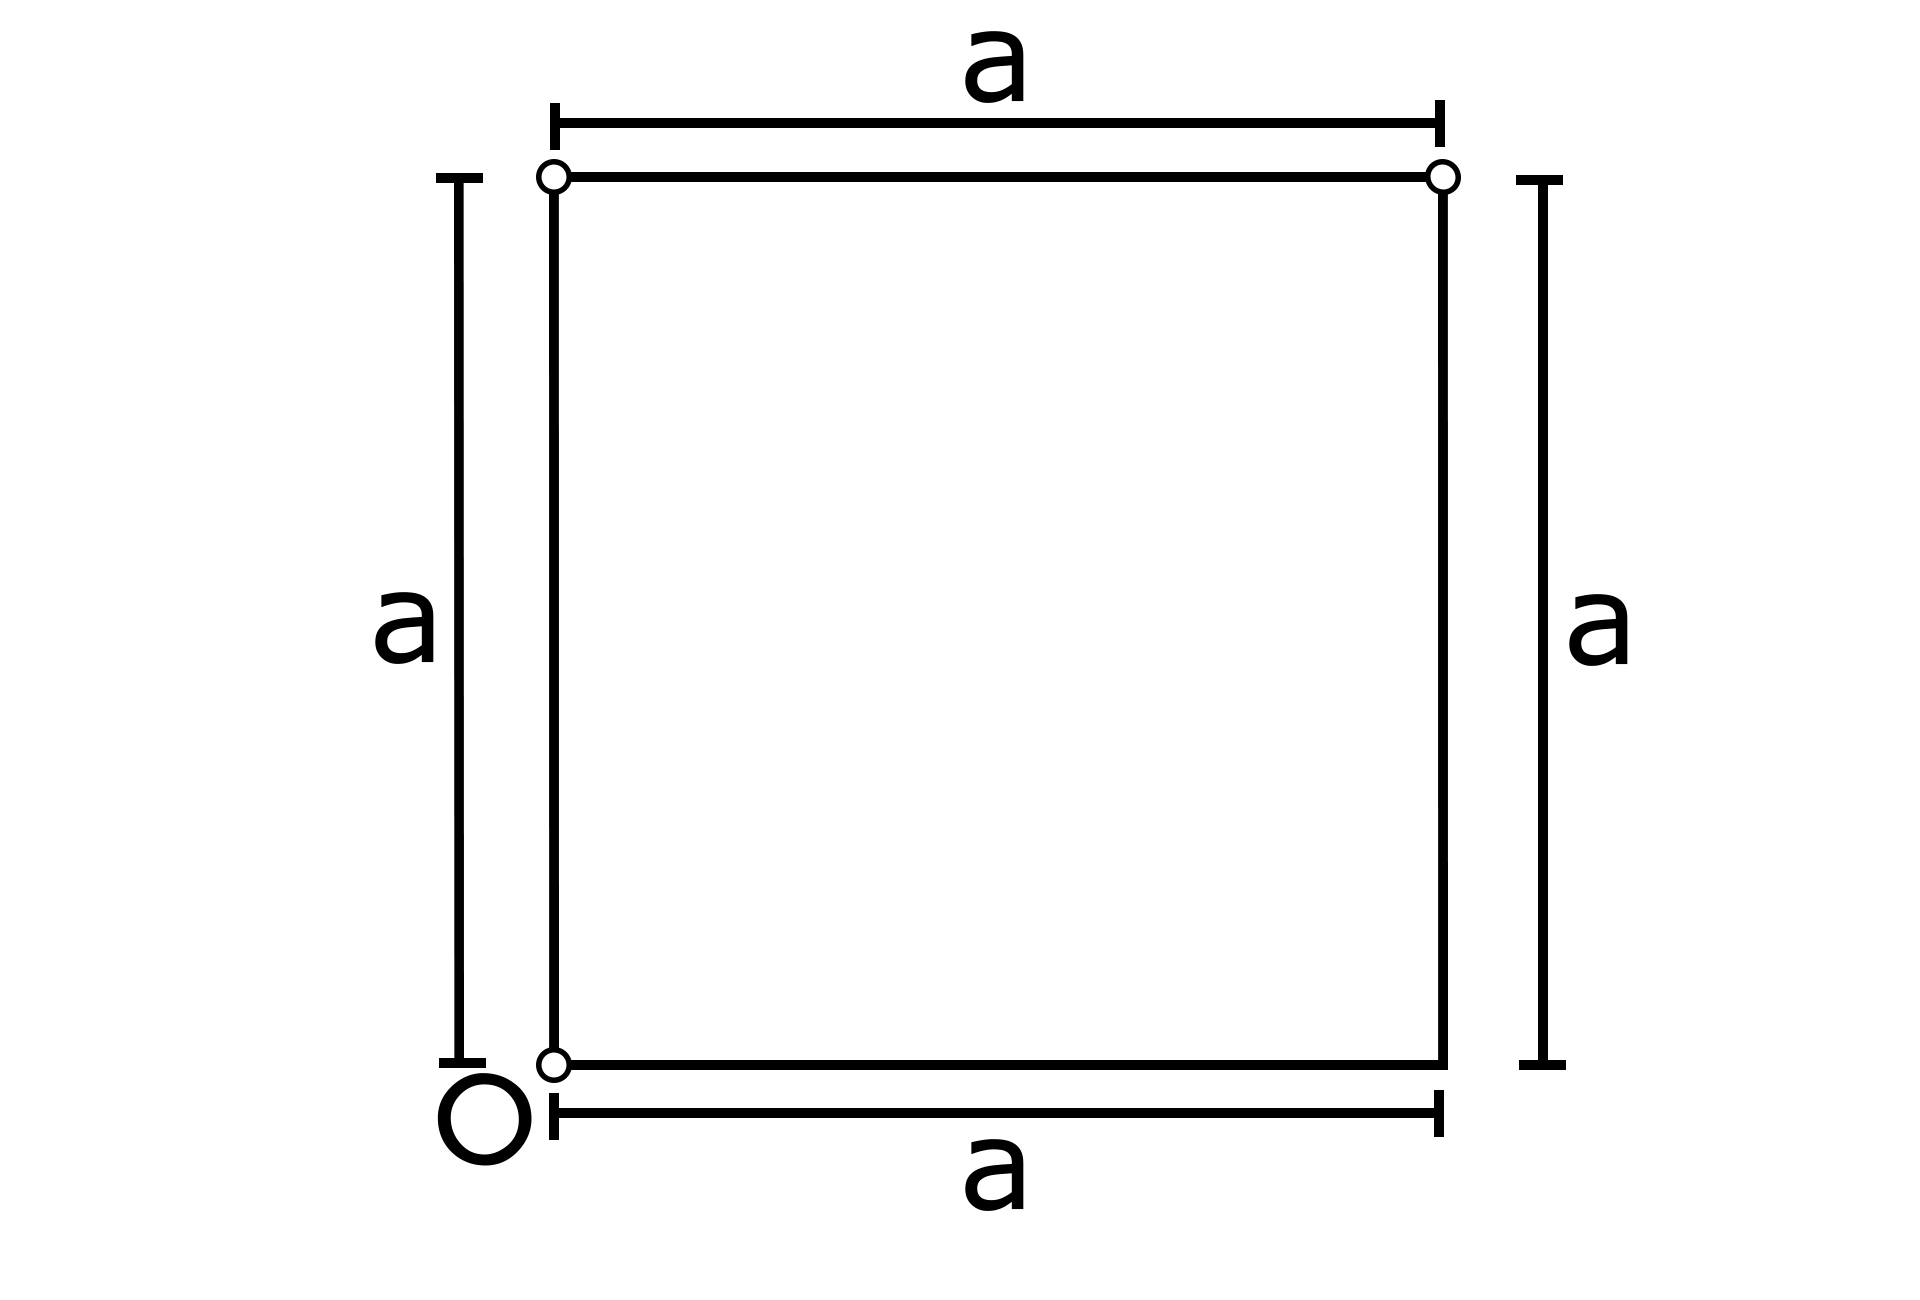
\includegraphics[width=0.95\textwidth]{Figures/Cuad10}
\caption[Trazado del último lado de la figura.]{Trazado del última lado de la figura.}
\label{fig:TrazFig10}
\end{figure}

Así, se tiene un cuadro de tamaño $a$ en cada lado para poder realizar las mediciones del sistema.

\section{Procedimiento}

Una vez trazada la figura, se identificará la localización de un punto cercano al trazado en coordenadas de latitud y longitud bajo el marco de referencia terrestre, tomando a Google Maps como herramienta de apoyo, para ahí configurar y colocar la estación base. Los lados de la figura se segmentarán en partes iguales, puntos en donde se realizará la medición de coordenadas de GPS durante la rutina.\\

Una vez verificados los cálculos, el sistema RTK será puesto en marcha con la estación base en un punto cercano con una vista libre del cielo, y el \textit{rover} en el vértice de la figura con posición conocida. Tras el paso de cierto tiempo en que el sistema se estabilice, se comenzará el recorrido de la figura.\\

En la memoria de la BeagleBone Black, se guardará un registro de las posiciones, calculadas por RTKLIB, del \textit{rover}, mismas que serán utilizadas para determinar el ajuste a una línea recta de los lados de la figura mediante regresión lineal.

\section{Conclusión}

Una vez conocidas las características del experimento a realizar, se procede a la realización de las pruebas, y al análisis de los datos obtenidos.\\

En el capítulo \ref{Chap:Res} se mostrarán datos del experimento de evaluación empleado y un análisis de los mismos.